\documentclass[border=10pt]{standalone}
\usepackage[utf8]{inputenc}
\usepackage{nacal}
\usepackage{tikz}
\usetikzlibrary{arrows.meta}
\def\Moneda{blue!75!white}
\def\Punto{red!60!black}
\begin{document}
\begin{tikzpicture}[x=9cm, y=0.9cm, every node/.style={font=\small}]
  % tres paneles: X_1, X_2, X_3 ; fila base de cada panel
  \foreach \n/\base in {1/4.4, 2/2.2, 3/0}{
    % ejes
    \draw[gray!60] (0,\base) -- (1,\base);
    \draw[gray!60] (0,\base) -- (0,\base+1.35);
    \node[anchor=east,\Moneda!80!black] at (-0.02,\base+0.6) {$X_{\n}$};
    \node[anchor=east,gray] at (-0.005,\base) {\scriptsize$0$};
    \node[anchor=east,gray] at (-0.005,\base+1) {\scriptsize$1$};
    % marcas diadicas de orden n
    \pgfmathsetmacro{\m}{2^\n}
    \pgfmathsetmacro{\mm}{\m-1}
    \foreach \j in {1,...,\mm}{
      \pgfmathsetmacro{\xx}{\j/\m}
      \draw[gray!50,dashed,thin] (\xx,\base) -- (\xx,\base+1.2);
    }
    % la funcion: 0 en los intervalos impares, 1 en los pares
    \foreach \j in {1,...,\m}{
      \pgfmathsetmacro{\xa}{(\j-1)/\m}
      \pgfmathsetmacro{\xb}{\j/\m}
      \pgfmathsetmacro{\v}{mod(\j,2)==0 ? 1 : 0}
      \draw[\Moneda,very thick] (\xa,\base+\v) -- (\xb,\base+\v);
      \fill[\Moneda] (\xa,\base+\v) circle (1.1pt);
      \ifnum\j=\m \fill[\Moneda] (\xb,\base+\v) circle (1.1pt);
      \else \draw[\Moneda,fill=white,thin] (\xb,\base+\v) circle (1.1pt); \fi
    }
  }
  % etiquetas del eje horizontal (solo abajo)
  \foreach \xx/\lab in {0/$0$, 0.125/$\tfrac18$, 0.25/$\tfrac14$, 0.375/$\tfrac38$, 0.5/$\tfrac12$, 0.625/$\tfrac58$, 0.75/$\tfrac34$, 0.875/$\tfrac78$, 1/$1$}{
    \node[anchor=north,gray!80!black] at (\xx,-0.12) {\scriptsize\lab};
  }
  \node[anchor=north,gray!80!black] at (0.5,-0.55) {\scriptsize$\omega$};
  % el suceso elemental omega = 0,3 = 0,0100... en binario
  \draw[\Punto,dotted,thick] (0.3,-0.05) -- (0.3,5.75);
  \node[anchor=south,\Punto] at (0.3,5.75) {$\omega=0{,}3$};
  \fill[\Punto] (0.3,4.4+0) circle (1.6pt);
  \fill[\Punto] (0.3,2.2+1) circle (1.6pt);
  \fill[\Punto] (0.3,0+0) circle (1.6pt);
  \node[anchor=west,\Punto] at (0.31,4.4+0.25) {\scriptsize$X_1(0{,}3)=0$};
  \node[anchor=west,\Punto] at (0.31,2.2+1.25) {\scriptsize$X_2(0{,}3)=1$};
  \node[anchor=west,\Punto] at (0.31,0+0.25) {\scriptsize$X_3(0{,}3)=0$};
\end{tikzpicture}
\end{document}
